\documentclass{article}
\usepackage{tikz}
\usepackage{adjustbox}

\begin{document}

\begin{adjustbox}{center}
    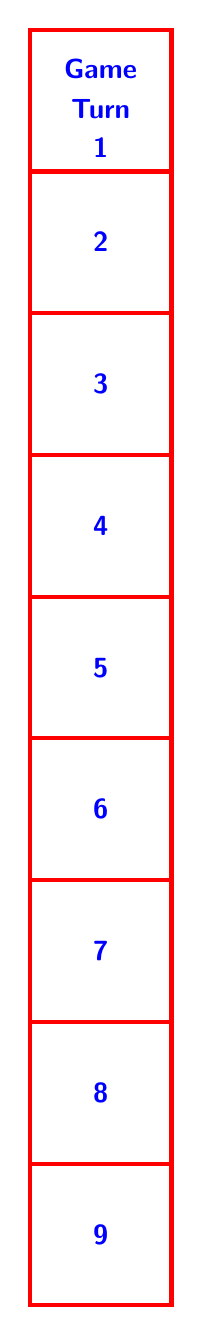
\begin{tikzpicture}

  % Define the gray color matching SVG default gray
  \definecolor{svggray}{RGB}{128,128,128}
  
  % Apply to everything
  \tikzset{every picture/.style={color=red}}

  \tikzset{every node/.style={text=blue}, every path/.style={draw=red}}


    % Define box properties
    \def\boxwidth{1.8}
    \def\boxheight{1.8}
    \def\boxthickness{1.5pt} % Adjustable line thickness

    % Define Game Turn numbers (2 to 9, since 1 is in the title box)
    \def\gameturns{2, 3, 4, 5, 6, 7, 8, 9}

    % First box with "Game Turn 1"
    \draw[line width=\boxthickness] (0, 0) rectangle (\boxwidth, -\boxheight);
    \node at (0.9, -0.5) {\sffamily \bfseries Game};
    \node at (0.9, -1.0) {\sffamily \bfseries Turn};
    \node at (0.9, -1.5) {\sffamily \bfseries 1};

    % Draw boxes and numbers for turns 2-9
    \foreach \x [count=\i] in \gameturns {
        \pgfmathsetmacro\ypos{-\i * \boxheight} % Calculate vertical position
        \draw[line width=\boxthickness] (0, \ypos) rectangle (\boxwidth, \ypos - \boxheight);
        \node at (0.9, \ypos - 0.9) {\sffamily \bfseries \x}; % Centered inside box
    }
\end{tikzpicture}

% \begin{tikzpicture}
%     % Define box properties
%     \def\boxwidth{1.8}
%     \def\boxheight{1.8}
%     \def\boxthickness{1.5pt} % Adjustable line thickness

%     % Define Game Turn numbers (2 to 9, since 1 is in the title box)
%     \def\gameturns{2, 3, 4, 5, 6, 7, 8, 9}

%     % First box with "Game Turn 1"
%     \draw[line width=\boxthickness] (0, 0) rectangle (\boxwidth, -\boxheight);
%     \node at (0.9, -0.5) {\sffamily \bfseries Game};
%     \node at (0.9, -1.0) {\sffamily \bfseries Turn};
%     \node at (0.9, -1.5) {\sffamily \bfseries 1};

%     % Draw boxes and numbers for turns 2-9
%     \foreach \x [count=\i] in \gameturns {
%         \pgfmathsetmacro\ypos{-\i * \boxheight} % Calculate vertical position
%         \draw[line width=\boxthickness] (0, \ypos) rectangle (\boxwidth, \ypos - \boxheight);
%         \node at (0.9, \ypos - 0.9) {\sffamily \bfseries \x}; % Centered inside box
%     }

% \end{tikzpicture}
\end{adjustbox}

\end{document}

